\chapter{Chapter 3 --- Research Design}\label{chapter-3-research-design}

This chapter states the design of the study as a whole: how the five
phases fit together, what data they run on, how the SZZ variants were
produced, what is measured and with what statistical protocol, and which
validity threats were anticipated in advance rather than discovered
afterwards.

The design has one organising commitment. \textbf{Every claim is a
paired comparison at the project level, and every reported number is
regenerable from committed inputs by a named script.} The remainder of
this chapter is largely an elaboration of what that commitment required.

\section{3.1 The phase pipeline}\label{the-phase-pipeline}

Each phase consumes the previous phase's output, and the dependencies
are data dependencies rather than narrative ones.

\begin{verbatim}
                 JIT-Defects4J reference labels
                              |
        +---------------------+----------------------+
        |                                            |
   [PHASE 1] -- six SZZ variants ----------+         |
   label quality                           |         |
        |                                  |         |
        +-- \ensuremath{\rho}\ensuremath{_0}, \ensuremath{\rho}\ensuremath{_1} per variant ------------+---------+--> [PHASE 3]
        |   (phase1_bias.json)             |         |    noise injection
        |                                  v         v    + repair
        +-- per-commit labels --------> [PHASE 2] -------> mechanism
                                        downstream              |
                                        impact                  |
                                                                v
                                                          [PHASE 4]
                                                          noise-aware
                                                          method
\end{verbatim}

\begin{itemize}
\tightlist
\item
  \textbf{Phase 1} measures how far each SZZ variant departs from the
  reference, and in which direction. Output: per-commit labels, and the
  flip-rate pair (\ensuremath{\rho}\ensuremath{_0}, \ensuremath{\rho}\ensuremath{_1}) per variant.
\item
  \textbf{Phase 2} trains models on each label source and evaluates them
  under four regimes of increasing realism, against two scoring
  conventions. Output: the inflation ladder and the label-source
  penalty.
\item
  \textbf{Phase 3} uses Phase 1's flip rates to inject calibrated noise
  into clean labels, and separately repairs real SZZ labels one error
  type at a time. Output: which error type costs the learner, and the
  mechanism.
\item
  \textbf{Phase 4} builds and pre-registers a method targeting whatever
  Phase 3 identifies.
\item
  \textbf{Phase 5} registers the alternative that Phase 4's exploratory
  analysis surfaced, and tests it on the noise-injection grid --- data
  generated \emph{after} the registration was committed, so the
  hypothesis is not tested on the sample that produced it.
\end{itemize}

\textbf{The dependencies between phases are genuine and were exercised
twice.} Phase 4's original design targeted false negatives; Phase 3
showed that error costs nothing, and Phase 4's registration was
rewritten before its first run. Phase 5 exists because Phase 4's
exploratory analysis surfaced a better-performing arm that could not
legitimately be promoted on the data that surfaced it. Had the phases
been planned in parallel rather than in sequence, neither correction
could have happened.

\section{3.2 Data}\label{data}

\subsection{3.2.1 Corpus}\label{corpus}

\begin{longtable}[]{@{}
  >{\raggedright\arraybackslash}p{(\linewidth - 2\tabcolsep) * \real{0.5000}}
  >{\raggedright\arraybackslash}p{(\linewidth - 2\tabcolsep) * \real{0.5000}}@{}}
\toprule\noalign{}
\endhead
\bottomrule\noalign{}
\endlastfoot
Projects & 21 Apache Java repositories \\
Commits & 27,319 \\
Reference defect-introducing & 2,332 (\textbf{8.54\%}) \\
Range per project & 544--4,026 commits; 19--335 defects; 1.8\%--19.3\%
defect rate \\
Features & The 14 Kamei change-level metrics \\
\end{longtable}

Projects were not selected by us. The corpus is JIT-Defects4J as
published, adopted whole so that the selection cannot be tuned to the
results. Its consequences for external validity are stated in \S{}3.5 and
Chapter 8.

\subsection{3.2.2 The reference labels}\label{the-reference-labels}

\texttt{label\_oracle} derives from JIT-Defects4J (Ni et al., ESEC/FSE
2022), an extension of LLTC4J (Herbold et al.). Its provenance was
traced through the repository and confirmed against the source paper
rather than assumed:

\begin{longtable}[]{@{}
  >{\raggedright\arraybackslash}p{(\linewidth - 2\tabcolsep) * \real{0.5000}}
  >{\raggedright\arraybackslash}p{(\linewidth - 2\tabcolsep) * \real{0.5000}}@{}}
\toprule\noalign{}
\begin{minipage}[b]{\linewidth}\raggedright
Step
\end{minipage} & \begin{minipage}[b]{\linewidth}\raggedright
Evidence
\end{minipage} \\
\midrule\noalign{}
\endhead
\bottomrule\noalign{}
\endlastfoot
\texttt{label\_oracle} & = \texttt{is\_buggy\_commit} in the published
feature pickles \\
The pickles & from the JIT-Fine replication package on Zenodo \\
Corpus check & the paper's own table reports 2,332 / 27,319 = 8.54\% and
matches this corpus \textbf{project by project} \\
\end{longtable}

\textbf{Construction, stated precisely because every downstream claim
depends on it.} Lines within bug-fixing commits were annotated manually,
retained only where at least three participants agreed;
\texttt{git\ blame} was then applied to those verified lines to identify
the introducing commit; everything else is clean by residual.

The reference is therefore \textbf{\texttt{git\ blame} seeded with
human-verified fix lines}, not manually verified ground truth for
defect-introducing commits. The phrase ``developer-verified ground
truth'' is inaccurate and is not used in this thesis. Chapter 4 \S{}4.1.1
develops the three consequences; the most important is that all measured
noise is a \textbf{lower bound}, because blame error is present on both
sides of every comparison and cancels.

\subsection{3.2.3 Features and
preprocessing}\label{features-and-preprocessing}

The 14 Kamei metrics are taken as published rather than recomputed, so
that feature extraction cannot differ between the reference and the
variants. Commits are deduplicated on (project, commit hash) and sorted
by author timestamp, which defines the stream order for every temporal
regime.

The pipeline was restructured so that two bulky inputs --- a 101 MB
archive and 830 MB of cloned repositories --- are replaced by two small
committed derived files (4.2 MB and 0.37 MB). The entire study therefore
runs on a continuous-integration runner from committed inputs, which is
what makes the reproducibility claim in \S{}3.6 checkable rather than
aspirational.

\subsection{3.2.4 Verification latency}\label{verification-latency}

Reconstructing when a defect label would actually have become known
requires the author date of each bug-fixing commit. These were extracted
once from the cloned repositories and committed as a small table. For
each variant, a commit's arrival time is the date of the fix that blamed
it; the union across variants supplies the reference condition's arrival
times.

\begin{figure}
\centering
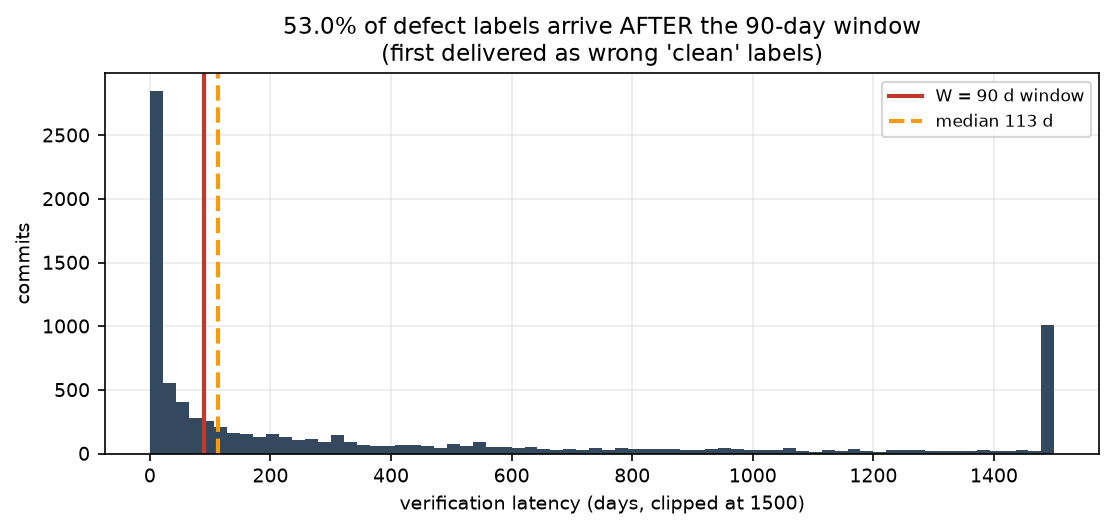
\includegraphics[width=\linewidth,keepaspectratio]{reports/figures/f6_latency.png}
\label{fig:f6_latency}
\caption{Distribution of verification latency against the 90-day
decision window}
\end{figure}

\textbf{Figure 3.1 --- Reading the figure.} How long after a commit its
defect label actually becomes available. The red line marks the 90-day
decision window; the orange dashed line the median, at 113 days.
\textbf{Over half the distribution lies to the right of the red line.}
Those labels arrive too late to be used inside the window, and are first
delivered to the learner as \emph{wrong clean labels}.

\textbf{This is the study's central construct-validity threat and is
declared here rather than in a footnote.} The published reference labels
carry no native fix-to-inducing linkage, so the reference condition is
blame-derived in \emph{construction} and \textbf{SZZ-derived in
\emph{timing}}. A coverage sensitivity analysis (67.8\% \ensuremath{\rightarrow} 100\% linkage)
bounds part of the exposure; it does not address the timing itself.
Every streaming result in Chapters 5--7 inherits this threat.

\section{3.3 SZZ variant
implementations}\label{szz-variant-implementations}

Six variants were produced with \textbf{PySZZ v2} (Rosa et al., JSS
2023), the reference implementation released with the
developer-informed-oracle study. Using the authors' own implementation
rather than a reimplementation removes one source of unexplained
variation, at the cost of inheriting whatever its defaults encode --- a
trade recorded here as a decision rather than left implicit.

Each variant was run on the same fix-commit set, and its output aligned
to the reference over an \textbf{identical 27,319-commit denominator}.
Partial denominators are a known source of incomparability: a variant
emitting fewer candidates can appear more precise merely by being scored
on a smaller population.

\subsection{3.3.1 The label-consistency
gate}\label{the-label-consistency-gate}

Mid-project it emerged that the Phase 2 dataset cache had gone stale
relative to a Phase 1 label regeneration. Models had been trained on
labels one commit older than the noise rates being reported, affecting
1.0--6.5\% of commits per variant. The root cause was an unguarded cache
keyed on modification time.

The remediation was three-part: a \textbf{content-hash staleness guard},
a \textbf{provenance sidecar} recording the SHA-256 of every label file
used to build the dataset, and an automated \textbf{consistency gate}
that recomputes the confusion matrix from the training data and asserts
it matches the reported noise rates for all six variants. The gate runs
in CI \textbf{before any compute is spent}, so a mismatch costs two
minutes rather than several hours. It was verified in both directions:
it fails on the stale data and passes on the corrected data.

This is recorded in the thesis rather than quietly fixed. A study about
label-provenance fragility encountered exactly that fragility in its own
pipeline, and now ships an executable assertion against its recurrence.

\section{3.4 Metrics and statistical
protocol}\label{metrics-and-statistical-protocol}

\subsection{3.4.1 Metric selection}\label{metric-selection}

\textbf{MCC is primary.} At an 8.54\% positive rate, accuracy is
uninformative: a model predicting ``clean'' for every commit scores
91.5\% accuracy and 0.0 MCC. MCC uses all four confusion-matrix cells
and is near zero for any uninformed strategy, which makes it the
appropriate primary under this imbalance. \textbf{G-mean} is reported
alongside as the geometric mean of per-class recalls, since it is
sensitive to abandoning the minority class in a way MCC partially shares
but expresses differently. \textbf{Cohen's \ensuremath{\kappa}} is used for agreement
between labelling procedures, where the question is concordance rather
than prediction.

\subsection{3.4.2 The prequential
estimator}\label{the-prequential-estimator}

Under streaming evaluation the metric is a trajectory, not a scalar, and
summarising it requires a choice. Two summaries are computed throughout:

\begin{itemize}
\tightlist
\item
  \textbf{Terminal fading} --- a confusion matrix with exponential
  forgetting (fading 0.99, effective window \ensuremath{\approx} 100 commits), read at end
  of stream.
\item
  \textbf{Time-averaged} --- the mean of the MCC trajectory over the
  stream.
\end{itemize}

\textbf{Neither is canonical, and this thesis does not claim otherwise.}
MCC is not a decomposable loss, so the prequential-with-fading
construction does not extend to it directly; of the two, the terminal
value is the closer analogue. The time-averaged value is treated as
\textbf{primary on a measured basis} --- roughly half the project-level
variance (0.051 against 0.092) --- not by appeal to a standard. An
earlier version of this work described it as ``the standard estimator'',
which was wrong and is corrected.

Both are reported for every streaming result. They agree on every
comparison in this thesis except one, which is named where it occurs.

\subsection{3.4.3 The unit of analysis}\label{the-unit-of-analysis}

\textbf{Every test is paired at the project level, \emph{n} = 21 (or 18
in Phase 4, after held-out exclusion), with seeds averaged before
pairing.} Seeds control model initialisation and fold randomness; they
are not independent observations. Pooling over the full record count
would be pseudo-replication, and is the first objection a methodologist
would raise.

\subsection{3.4.4 Effect sizes}\label{effect-sizes}

Each comparison reports:

\begin{itemize}
\tightlist
\item
  \textbf{Wilcoxon signed-rank \emph{p}} --- paired, distribution-free.
\item
  \textbf{Matched-pairs rank-biserial correlation} --- derived from the
  same signed ranks as the \emph{p}-value, so the effect size and the
  test agree by construction. It reads as \emph{consistency}: +1.000
  means every project moved in the same direction.
\item
  \textbf{Hodges--Lehmann estimator} --- the median of pairwise Walsh
  averages, the location estimate that accompanies the signed-rank test.
\item
  \textbf{Percentile bootstrap confidence interval}, computed
  \textbf{for the Hodges--Lehmann statistic itself}, with the statistic
  recomputed inside every resample.
\end{itemize}

Two of these are corrections to an earlier protocol and are recorded as
such. Cliff's \ensuremath{\delta} was initially computed \emph{unpaired}, all-versus-all
with denominator \emph{n}\ensuremath{\cdot}\emph{m}, discarding the pairing the design
exists to preserve; on the headline comparison it reported 0.74 where
the paired statistic reports +1.000. Separately, the bootstrap
originally resampled the median while the Hodges--Lehmann estimate was
reported beside it --- an interval for a different quantity than the
point estimate.

\subsection{3.4.5 Multiplicity}\label{multiplicity}

Seventy-four tests are run in Phase 2 alone. Multiplicity is corrected
\textbf{twice}:

\begin{itemize}
\tightlist
\item
  \textbf{Holm within test family} --- families grouped by the
  comparison being made.
\item
  \textbf{Holm globally across all tests} --- no family argument
  required.
\end{itemize}

The global column exists because the families were defined \emph{during}
analysis, not declared in advance. A sceptic can reasonably argue the
grouping was chosen to help the results; \textbf{a claim surviving
global Holm needs no defence of how families were drawn.} Every headline
claim in this thesis survives the global column, and where a claim
survives only within-family correction, that is stated.

\subsection{3.4.6 Pre-registration}\label{pre-registration}

\textbf{Phases 1--3 are exploratory.} Their hypotheses were formed
during analysis and every result is labelled accordingly; the global
multiplicity correction is the sensitivity analysis that makes them
defensible without a pre-registration.

\textbf{Phases 4 and 5 are pre-registered}, with hypotheses, primary
model, acceptance bar and correction committed to version control before
each first run. Phase 4's registration was revised once, after Phase 3
refuted the hypothesis it was built on and while Phase 4 still had zero
results --- the only point at which revision is legitimate. Phase 5's
registration is separate, and was deliberately aimed at data that did
not exist when it was written. Chapter 7 \S{}7.1 and \S{}7.5 give the full
accounts.

\section{3.5 Threats to validity, framed in
advance}\label{threats-to-validity-framed-in-advance}

Stating the framework before the results appear is deliberate: it
prevents the threat list from being assembled to fit whatever was found.

\textbf{Construct validity.} The reference is \texttt{git\ blame} seeded
with verified fix lines, not ground truth, so comparisons isolate
tangling rather than total labelling error and measured noise is a lower
bound. Arrival times for the reference condition are SZZ-derived
(\S{}3.2.4) --- the single most serious threat in the study.

\textbf{Internal validity.} Temporal leakage is the threat the design
exists to expose, and is therefore a \emph{manipulated variable} rather
than a defect. Cache staleness is addressed by the gate (\S{}3.3.1). Repair
and injection experiments are oracle-assisted by construction and are
labelled as upper bounds, not methods.

\textbf{External validity.} One benchmark family: 21 Apache Java
repositories of a single dataset lineage. The corpus is SZZ-shaped,
since changes adding no new lines were excluded by the dataset authors,
so defects introduced purely by deletion cannot appear. Projects are
weighted equally despite an eighteen-fold range in defect count.

\textbf{Conclusion validity.} With 21 paired projects, effects below
roughly 0.04 MCC are not resolvable --- a limit that becomes
load-bearing for the latency decomposition, which is reported as
unresolved rather than as null. Multiplicity is corrected twice. The
number of exploratory comparisons is large, which is precisely why the
global correction is reported.

\textbf{One scope limit declared before Phase 3 ran.} Because the
reference labels are themselves blame output, every reference positive
is blame-reachable by construction. \textbf{No false negative measured
against this reference can be attributed to blame's structural inability
to trace a defect.} Phase 3 can therefore study false-negative noise
arising from over-filtering and seed-line divergence --- the two
mechanisms Chapter 4 shows are actually operating --- but can make no
claim about blame-unreachability. Declaring this in advance prevents an
unavailable explanation from being offered afterwards.

\section{3.6 Reproducibility}\label{reproducibility}

Every number in Chapters 4--7 is regenerable from committed inputs by a
named script, and the chapter-to-artefact mapping is explicit:

\begin{longtable}[]{@{}
  >{\raggedright\arraybackslash}p{(\linewidth - 4\tabcolsep) * \real{0.3333}}
  >{\raggedright\arraybackslash}p{(\linewidth - 4\tabcolsep) * \real{0.3333}}
  >{\raggedright\arraybackslash}p{(\linewidth - 4\tabcolsep) * \real{0.3333}}@{}}
\toprule\noalign{}
\begin{minipage}[b]{\linewidth}\raggedright
Chapter
\end{minipage} & \begin{minipage}[b]{\linewidth}\raggedright
Script
\end{minipage} & \begin{minipage}[b]{\linewidth}\raggedright
Principal outputs
\end{minipage} \\
\midrule\noalign{}
\endhead
\bottomrule\noalign{}
\endlastfoot
4 & \texttt{experiments/evaluate\_confusion\_matrix.py} & quality table,
\ensuremath{\kappa} matrix, \texttt{phase1\_bias.json} \\
5 & \texttt{experiments/run\_phase2\_impact.py} & regime \ensuremath{\times} label-source
matrix, 74 tests \\
6 & \texttt{experiments/run\_phase3\_noise.py},
\texttt{run\_phase3\_addendum.py} & dose curves, repair statistics, \ensuremath{\lambda}
traces \\
7 & \texttt{experiments/run\_phase4\_tuning.py},
\texttt{run\_phase4\_na\_orb.py} & frozen configuration, registered
tests \\
7 & \texttt{experiments/run\_phase5\_damping.py} & Phase 5 registration
and its five registered tests \\
Appendix & \texttt{experiments/run\_robustness\_checks.py} & project
table, floor sensitivity, mechanism test \\
\end{longtable}

Runtime dependencies are pinned to the exact versions every result was
computed with, so a runner reproduces the local environment rather than
approximating it. The label-consistency gate runs before every
experiment in CI.

The next four chapters report what these scripts produce.
